\chapter{Voltage-source converter}
\label{chp:VSC}

Finally, we can open the magical box that we previously just said converted the voltage from DC to AC. From what we see right away in \cref{fig:internals_of_VSC}, we see that the \gls{VSC} contains a \gls{PLL}, a \gls{PWM}, a controller, as two blocks performing the Park and the inverse Park transform. From what we have seen up until now, the \gls{VSC} can affect the continuous circuit through three inputs $i_{dc}$, $v_{cv,d}$ and $v_{cv,q}$. Intuitively power can not come from nowhere, so there exists one constraint as well. The resulting system has two degrees of freedom. If the controller has two degrees of freedom, it is in theory possible to make it follow two control objectives. 

\begin{figure}[ht]
 \centering
 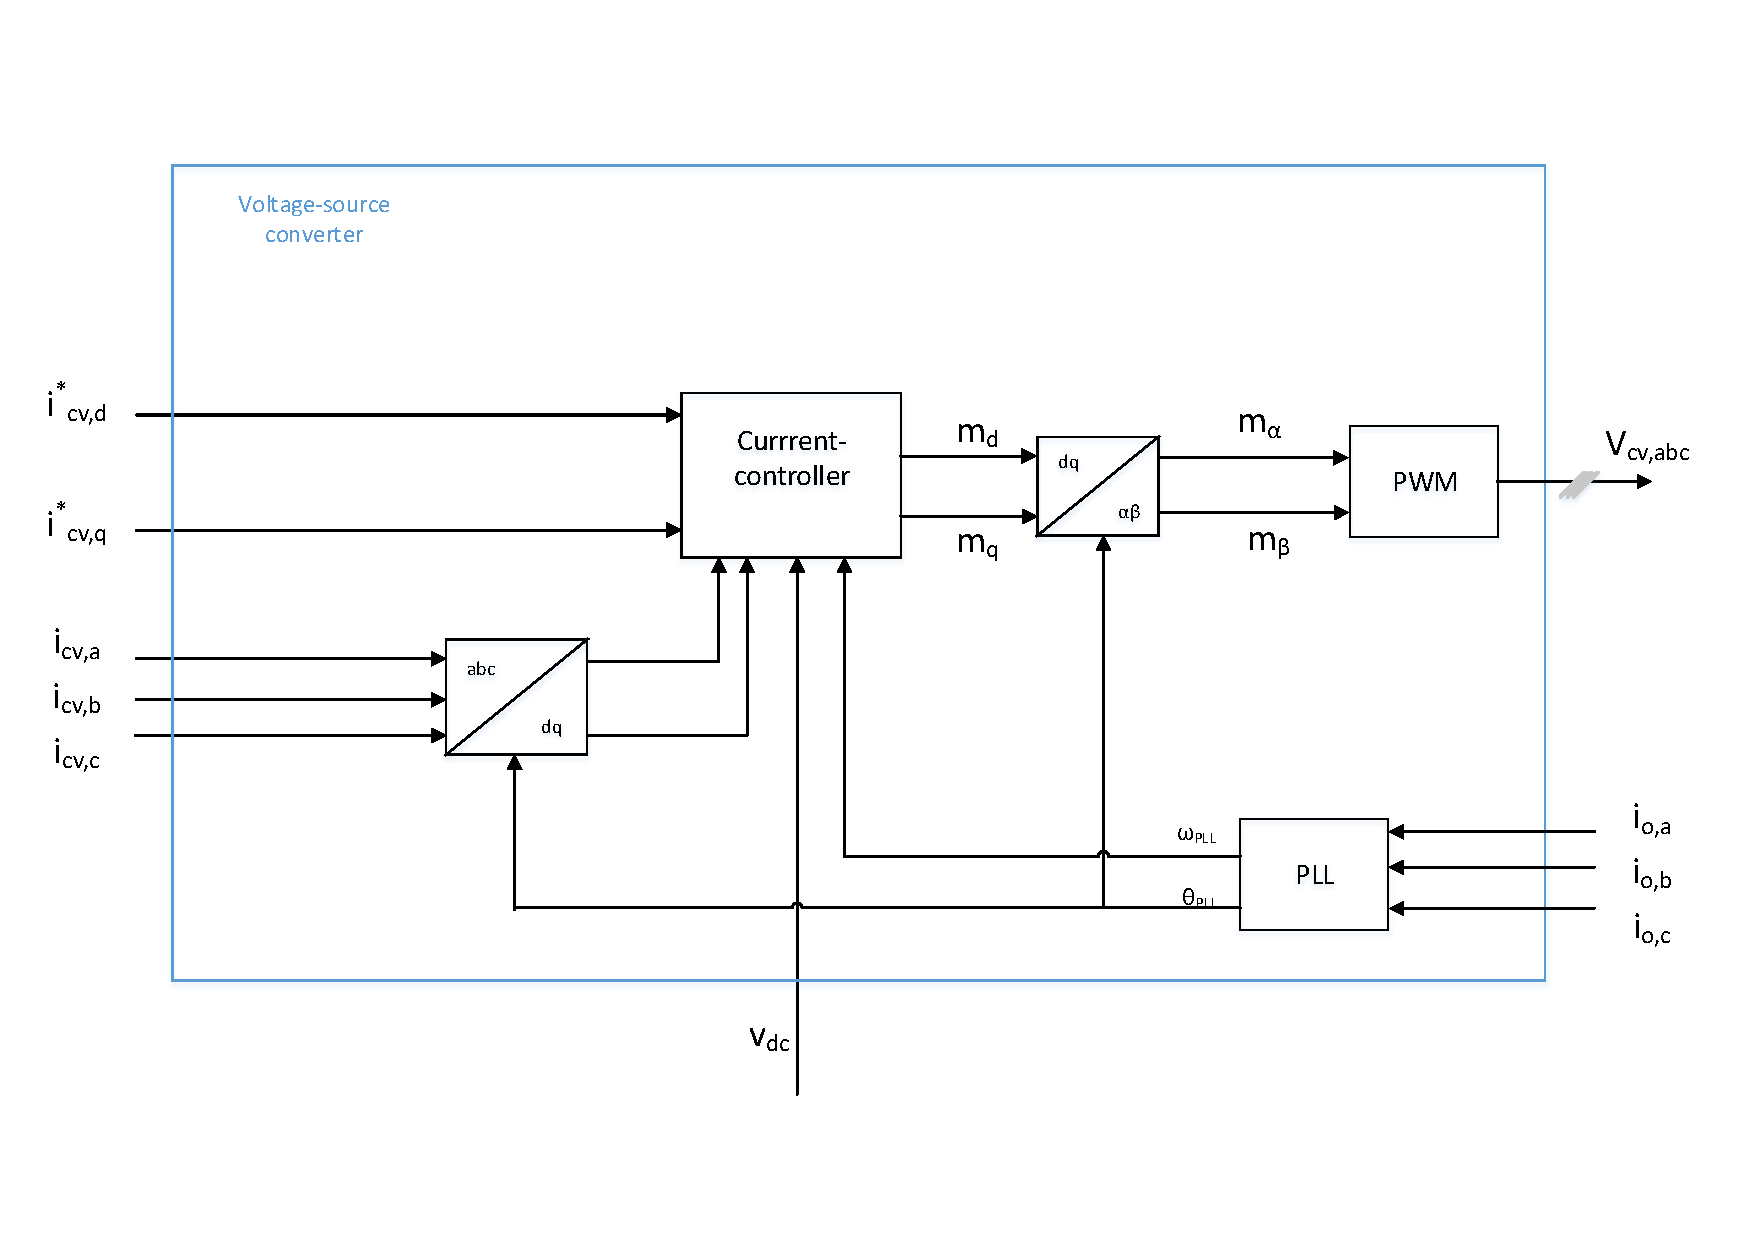
\includegraphics[width=\textwidth,height=\textheight,keepaspectratio]{Figures/Internals_of_the_converter.pdf}
 \caption{Voltage source converter (Inspired by \cite{Suul_electro_presentation_1})}
 \label{fig:internals_of_VSC}
\end{figure}{}
% \todo[inline]{Legg til nødvendig figur her}

As mentioned before, the \gls{VSC} contains a \gls{PWM}. A \gls{PWM} is described in more detail in \cref{sec:PWM}. But the short version of it is that it is able to give something that can almost follow a voltage reference by switching quickly between two voltages, which will give a smooth signal if it is passed through an RLC-filter. But the fact that the \gls{PWM} has to work on periodic cycles means that it has to be sampled. The time-delay in the system comes from the sampling that the \gls{PWM} has to do, as well as the sampling that is done to get the voltage and current measurements. 

\section{Phase Locked Loop (PLL)}
\label{sec:PLL}
In a grid, it is possible that the phase and frequency are not the same as what was first assumed when the system was designed. In order to remedy this, an estimate that tries to follow the actual phase of the grid has to be given instead. In order to do this, a PLL is used, which has a somewhat similar structure to a PI-controller, as seen in \cref{fig:PLL_fig}. The purpose of this controller is to reduce the perceived reactive voltage when using the estimated angle in order to transform the system from the $abc$ to the $dq$-frame. $atan2$ is a very non-linear mapping, so it makes more sense to filter both d and q before they are transformed into an angle by $atan2$. 

\begin{figure}
 \centering
 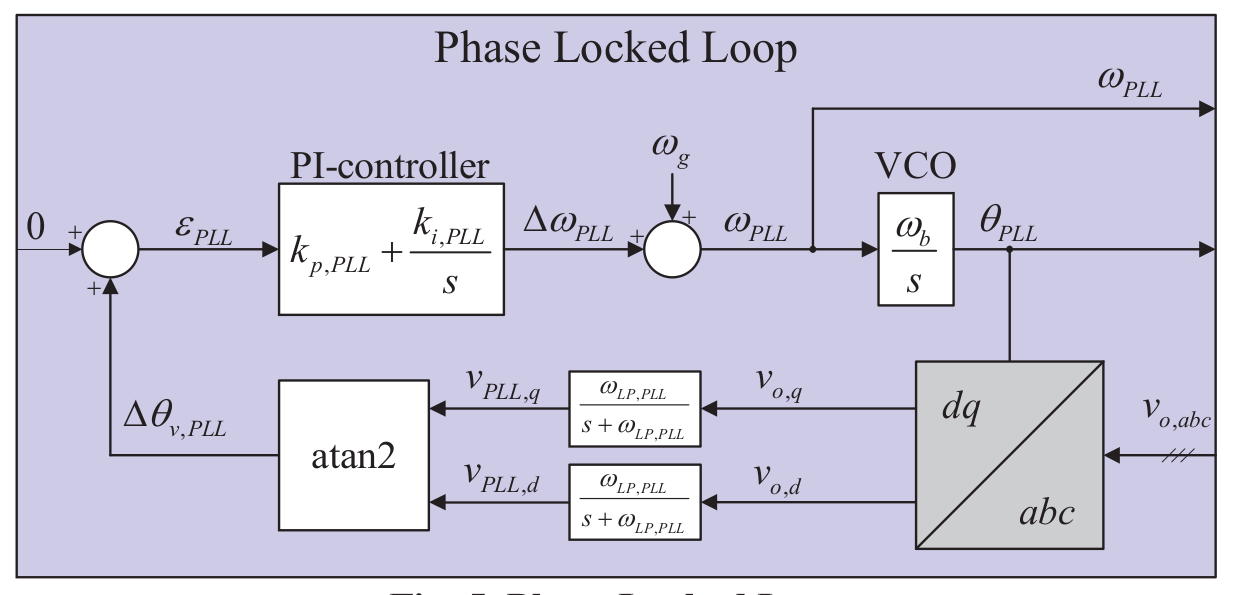
\includegraphics[width=\textwidth,height=\textheight,keepaspectratio]{Figures/PLL.png}
 \caption{Phase Locked Loop (\gls{PLL}), taken from \cite{Suul_paper_1,Suul_electro_presentation_1}}
 \label{fig:PLL_fig}
\end{figure}{}
 
Also worth noting is the term $\omega_g$, which is a result of fact that the controller is based on linearization around the expected operating frequency $\omega_g$. 

One final point to take special note of is the fact that the regulator uses the estimate $\omega_{PLL}$ for some feed-forward terms. Therefore, it is quite possible that the system may experience nonlinear characteristics as a result of the PLL. 

\section{Current-controller}

It is possible to have several different kinds of regulators, depending on what is needed. It is possible to regulate the active power on the AC-side, or the ammount of current drawn on the DC-side. Usually, these are controlled by giving some kind of reference to a current controller. But in our case, the controller will simply be a current-controller with nothing more. Since the PWM only is able to take in signals saying how long it should stay at the high or low voltage, the output AC voltage will be proportional to the input DC voltage. Because of this, it can often be good to get the modulation index by dividing the desired voltage by the measured DC voltage. 
\noindent
\begin{figure}[ht]
 \centering
 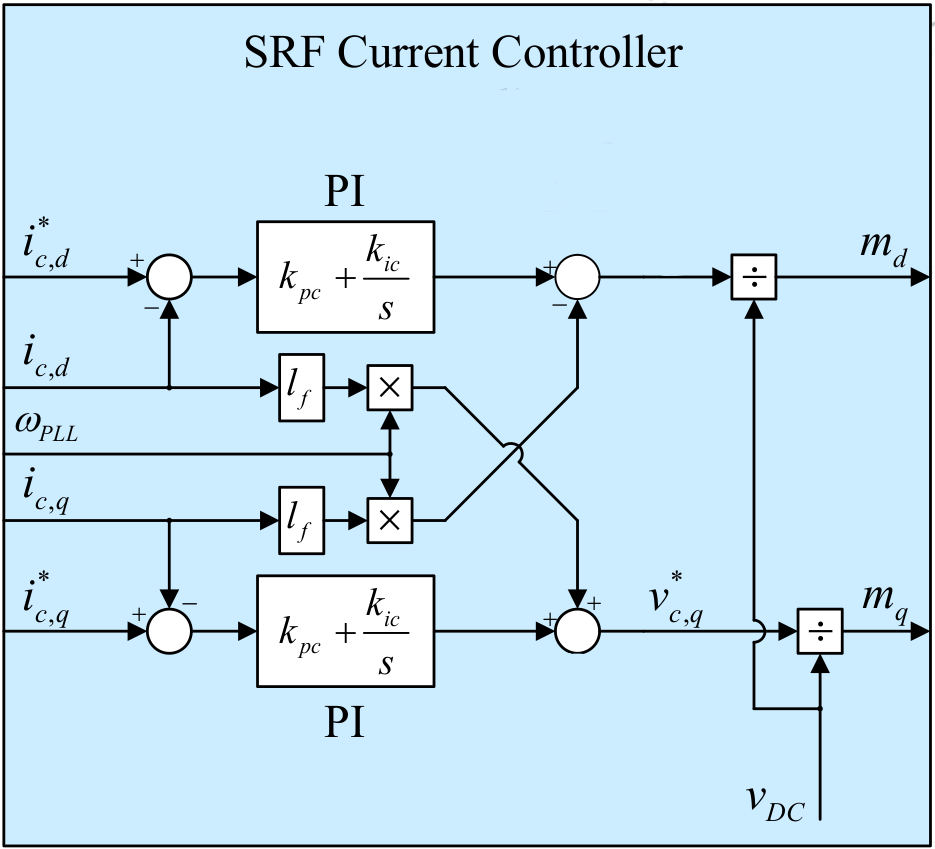
\includegraphics[width=\textwidth,height=\textheight,keepaspectratio]{Figures/stolen_controller_edit.png}
 \caption{Voltage source converter (Taken from \cite{Suul_electro_presentation_1,Suul_paper_1}, edited to reflect the equations used in this project)}
 \label{fig:decoupled_controller}
\end{figure}{}
When looking at the equations for the current in the controller, one term causes a lot of trouble. That term is $j\omega\gls{_g}\omega\gls{_b}\Vec{i_{cv}}$,since it couples the current in the d and q axis. This means that the d- and the q-current become them dependant on each other. In order to mitigate these problems, the decoupling terms $j l_f\omega_{PLL}$ are added. By adding the decoupling terms, the resulting matrix should become 
\begin{align}
 \frac{d \Vec{i\gls{_cv}}}{dt} &= \frac{\omega\gls{_b}}{l\gls{_f}}\Vec{v_{cv,PI}} + j\frac{\omega\gls{_b}}{l\gls{_f}}( l_f \omega_{PLL} ) - \frac{\omega_b}{l_f}\Vec{v}\gls{_o} - \left( \frac{r_{l_f}\omega_b}{l_f} + j\gls{omega_g}\omega_b \right) \Vec{i_{cv}}\\
\end{align}{}
So, if $\omega_{PLL} = \omega_g$ then, the terms will cancel, and the d and q-current will be decoupled. In theory, there are no guarantees that this will work perfectly, but in practice, it usually works quite well \cite{Suul_electro_presentation_1}
The remaining terms, which are represented by $\Vec{v_{cv,PI}}$ can be used by a PI-controller. The controllers can usually be tuned independently of each other. These can usually be tuned by Modulus optimum or symetrical optimum \cite{Suul_electro_presentation_1,Suul_paper_2}. In this case, the deviiation from a reference, for both active and reactive current is given as inputs to the controller. But, usually, if something else has to be controlled, a slower controller is normally used in order to give a reference to the current controller. 

\todo[inline]{Bør jeg legge til noe mer her? (Hvordan man tuner kontrollerne) }

